\documentclass{article} % For L/takaTeX2e
\usepackage{nips13submit_e,times}
\usepackage{hyperref}
\usepackage{amsmath}
\usepackage{amssymb}
\usepackage{amsthm}
\usepackage[]{graphicx}
\usepackage{subfig}

\newtheorem{theorem}{Theorem}
\newtheorem{lemma}{Lemma}
\newtheorem{corollary}{Corollary}

%\documentstyle[nips13submit_09,times,art10]{article} % For LaTeX 2.09

\newcommand{\X}{{\mathcal{X}}}
\newcommand{\R}{{\mathbb{R}}}
\newcommand{\N}{{\mathbb{N}}}
\newcommand{\E}{{\mathbb{E}}}

\title{Information Theoretic Clustering using Kernel Density Estimation}


\author{
Shashank Singh \\
Department of Statistics\\
Machine Learning Department\\
Carnegie Mellon University\\
Pittsburgh, PA 15213 \\
\texttt{sss1@andrew.cmu.edu} \\
\And
Bryan Hooi \\
Department of Statistics\\
Machine Learning Department \\
Carnegie Mellon University \\
Pittsburgh, PA 15213 \\
\texttt{bhooi@andrew.cmu.edu} \\
}

% The \author macro works with any number of authors. There are two commands
% used to separate the names and addresses of multiple authors: \And and \AND.
%
% Using \And between authors leaves it to \LaTeX{} to determine where to break
% the lines. Using \AND forces a linebreak at that point. So, if \LaTeX{}
% puts 3 of 4 authors names on the first line, and the last on the second
% line, try using \AND instead of \And before the third author name.

\newcommand{\fix}{\marginpar{FIX}}
\newcommand{\new}{\marginpar{NEW}}
\newcommand\norm[1]{\left\lVert#1\right\rVert}
\nipsfinalcopy

\begin{document}
\maketitle
\section{Introduction}
In recent years, information-theoretic clustering algorithms have been proposed
which assign data points to clusters so as to maximize the mutual information
between cluster labels and data
\cite{faivishevsky2010nonparametric,wang2011information}. Using mutual
information for clustering has several attractive properties: it is flexible
enough to fit complex patterns in the data, and allows for a principled
approach to clustering without assuming an explicit probabilistic generative
model for the data. 

Recently, \cite{steeg2013demystifying} showed examples in which maximizing
mutual information leads to poor performance when the clusters are unbalanced,
even in very simple cases. This occurs because algorithms that maximize mutual
information are biased toward splitting the data into equal-sized clusters, and
this causes the algorithms to perform poorly in the large data limit. They
propose to instead minimize the conditional entropy of the cluster labels given
the data, where conditional entropy is estimated using a nearest neighbor-based
approach. They show that minimizing this objective instead of maximizing mutual
information tends to select clusters with large gaps separating them rather
than simply selecting approximately equal-sized clusters.

In terms of computation, \cite{wang2011information} formulate the mutual
information maximization problem as a semidefinite program, and additionally
use a low rank inement heuristic to obtain low rank solutions.
\cite{steeg2013demystifying} apply a similar approach to minimizing conditional
entropy, involving a relaxation of the discrete cluster variables resulting in
a semidefinite program, which is then converted to a candidate solution by
rounding with respect to random projections, taking a similar approach to
\cite{goemans1995improved}.

The {\bf main contributions} of this work are to:
\begin{enumerate}
\item further motivate conditional entropy minimization as a clustering
objective using the principle of Minimum Description Length (MDL).
\item propose a principle for estimaing the number of clusters based on MDL.
\item propose a novel approach, CHMin, for minimizing the conditional entropy
using kernel density estimation and gradient descent.
\item draw a theoretical connection portraying CHMin as a refinement of the
$K$-means algorithm.
\item empirically study the performance of CHMin on some simple synthetic and
real datasets.
\end{enumerate}

\newpage
\section{Definitions and Preliminaries}
In the following, $x_1, \dots, x_n \in \mathbb{R}^d$ are the data points and $y_1, \dots, y_n \in \{1, \dots, K\}$ are the associated clustering variables. We first define our kernel-based density estimators. We use the usual density estimator for $X$:
\[ \hat{p}(x) := \frac{1}{hn}\sum_{j=1}^n K(\frac{x - x_j}{h}) \]
The estimator for joint density of $(X, Y)$ (where $Y$ has support $\{1, \dots, K\}$) is:
\[ \hat{p}(x, y) := \frac{1}{hn}\sum_{j=1}^n 1\{y_j=y\} K(\frac{x - x_j}{h}) \]
Let $C_k = \{i: Y_i = k\}$, the indices of points assigned to cluster $k$, and define $n_k = |C_k|$.\\
We estimate the density of $Y$ by its empirical distribution $\hat{p}(y) := \frac{n_y}{n}$.\\
The conditional density estimator of $X$ given $Y$ is
\[ \hat{p}(x | y) := \frac{\hat{p}(x, y)}{\hat{p}(y)} \]
We then define the estimated entropy of $X$:
\[\hat{H}(X) := - \frac{1}{n} \sum_{i=1}^n \log(\hat{p}(x_i)) \]
$\hat{H}(Y)$ and $\hat{H}(X|Y)$ are defined analogously (using $\hat{p}(y)$ and $\hat{p}(x | y)$ respectively).\\
Finally, we define
\begin{align*}
\hat{H}(Y|X) &:= \hat{H}(Y) + \hat{H}(X|Y) - \hat{H}(X) \\
&= -\frac{1}{n}\sum_{i=1}^n \log \hat{p}(y_i) -\frac{1}{n}\sum_{i=1}^n \log \hat{p}(x_i | y_i) + \frac{1}{n}\sum_{i=1}^n \log \hat{p}(x_i) \\
&= -\frac{1}{n}\sum_{i=1}^n \log \left( \frac{\hat{p}(x_i, y_i)}{\hat{p}(x_i)} \right)
\end{align*} 

\section{Conditional Entropy Minimization and Minimum Description Length}
In this section, we first show that conditional entropy minimization can be seen as a special case of model fitting using Minimimum Description Length (MDL). When using MDL, we select between competing models based on which model allows us to compress the data to the smallest number of bits, providing a trade-off between improving model fit and minimizing model complexity\cite{rissanen1978modeling}. \\\\
We represent the data using a two-part coding scheme, in which we encode a \textit{point hypothesis} (or probability distribution) $H \in \mathcal{H}$ using $L(H)$ bits, and then encode the data $D$ given hypothesis $H$, requiring $L(D | H)$ bits. We refer to $\mathcal{H}$, the set of hypotheses under consideration, as the \textit{model}. For example, $\mathcal{H}$ may consist of all mixture distributions of $K$ Gaussians. More generally, the following discussion applies to mixtures of any parametric family of distributions where the number of parameters needed to encode each cluster is fixed (for example, for mixtures of Gaussians, each cluster is encoded by its mean and covariance parameters). Moreover, we use the same parametric family when estimating entropy - that is, instead of using kernel density to estimate empirical distributions, we estimate density within each cluster as a distribution from the same parametric family (e.g. a Gaussian distribution), fitted using maximum likelihood. We also assume that the number of clusters $K$ is fixed.  \\\\
Given data $X$, under MDL we select the point hypothesis $H  = (Y, \mu)$ which minimizes the total description length $L(H) + L(X|H)$, where $Y$ contains the cluster assignments and $\mu=(\mu_1, \dots, \mu_K)$ contains the cluster parameters, e.g. cluster centers in a Gaussian mixture model.\\
\begin{theorem}
Under the above conditions, minimizing description length $L(H) + L(X|H)$ is equivalent to minimizing estimated conditional entropy $H(Y|X)$.
\end{theorem}
\begin{proof}
By assumption, encoding the cluster parameters $\mu$ requires a fixed number of parameters, so we can ignore this cost. It remains to encode the cluster assignments $Y$, requiring $L(Y)$ bits, and to encode the data given ths model, requiring $L(X|Y,\mu)$ bits. \\\\
We first compute $L(X|Y,\mu)$. By Shannon's source coding theorem, the optimal expected code length is achieved by assigning a code length of $-\log(p)$ to an outcome with probability $p$ (and an analogous fact holds for continuous distributions with $p$ as the density, by discretizing the space of outcomes to small intervals). As such, given hypothesis $H = (Y, \mu)$, the optimal code requires $\hat{p}(x_i | y_i)$ bits to represent $x_i$. This results in a code length of
\begin{align*}
L(X|Y,\mu) &= -\sum_{i=1}^n \log \hat{p}(x_i | y_i) \\
&= \hat{H}(X|Y)
\end{align*}
Next, we compute $L(Y)$. To encode the cluster assignments $Y$, we encode each $y_i$ with respect to the empirical distribution of $Y$, which by Shannon's source coding theorem results in a code length for $y_i$ of $-\log \hat{p}(y_i)$, and summing over $i$, the code length is
\begin{align*}
-\sum_{i=1}^n \log \hat{p}(y_i) = \hat{H}(Y)
\end{align*}
Note that a recipient of a message with $Y$ encoded in this way can infer which $y_i$ are in the same cluster based on which $y_i$ are encoded using the same code word, but they cannot infer how these code words correspond to the actual clusters parametrized by $\mu_1, \dots, \mu_k$. As such, we additionally need to send an additional $\log(K!)$ bits to encode which of the $K!$ possible permutations of the code words correspond to $\mu_1, \dots, \mu_K$ respectively. However, since $K$ is fixed, this is a constant and can be ignored.\\\\
Combining the above results, we find that the overall description length is:
\begin{align*}
L(H) + L(X|H) = \hat{H}(Y) + \hat{H}(X|Y) + \text{const}
\end{align*}
\end{proof}
One benefit of viewing conditional entropy minimization in the MDL framework is that we can select the number of clusters $K$ in a principled manner based on MDL. We will show that selecting the optimal model in this way amounts to minimizing conditional entropy plus a regularization-like term that penalizes the number of clusters $K$.\\\\
In the MDL approach to model selection, we define models $\mathcal{H}_1,
\mathcal{H}_2, \dots$, each of which is a set of point hypotheses. We select
the best model by encoding the data with respect to each model and selecting
the model that gives the best compression. In our case $\mathcal{H}_K$ is the
set of partitions into $K$ clusters. As before, the description length for model $\mathcal{H}_K$ is given by selecting point hypothesis $H \in \mathcal{H}_K$ to minimize $L(H) + L(X|H)$. However, the number of clusters $K$ is no longer fixed.
\begin{theorem}
To select the number of clusters $K$ by MDL, we minimize
\[
\hat{H}(Y|X) + \log^*(K) + Kd(\log(2B) + \frac{1}{2} \log(n)) + \log(K!)
\]
\end{theorem}
\begin{proof}
Encoding the data requires encoding the number of clusters $K$, the cluster parameters $\mu$, the cluster assignments $Y$, and the data $X$ given $Y$ and $\mu$.\\\\
To encode $K$, we use Rissanen's ``universal code for the natural numbers," which was shown by Rissanen to achieve close to the shortest possible code length for large natural numbers \cite{rissanen1983universal}. Define the $\log^*$ function as $\log^*(n) = \log_2(n) + \log_2 \log_2 (n) + \dots$, where only the positive terms are to be included in the sum. Then this code length of $K$ is
\[ L(K) = \log^*(K) + \log_2(K_0) \]
where $K_0$ is a constant (equal to $\sum_{n>1} 2^{-\log^*(n)}$). \\\\
Next, we compute $L(\mu)$. Since the $\mu_i$ are continuous, we need to discretize them before encoding them: following \cite{rissanen1983universal}, we use a precision of $1/\sqrt{n}$, the asymptotic error of estimating each parameter: this choice was shown to be optimal for regular parametric families in \cite{rissanen1983universal}. Assuming that each parameter $\mu_i$ has dimension $d$ and that the cluster centers are in a bounded range $|\mu_i| \le B$, the parameters consist of $Kd$ numbers, each taking one of $2B\sqrt{n}$ possible values after discretization, so the code length is:
\begin{align*}
L(\mu) &= Kd \log(2B\sqrt{n}) \\
&= Kd(\log(2B) + \frac{1}{2} \log(n))
\end{align*}
Combining this with the previous theorem, the overall description length is:
\begin{align*}
L(X|H) + L(H) &= \hat{H}(Y) + \hat{H}(X|Y) +\log^*(K) + Kd(\log(2B) + \frac{1}{2} \log(n)) + \log(K!) +  \text{const}\\
&= \hat{H}(Y|X) + \log^*(K) + Kd(\log(2B) + \frac{1}{2} \log(n)) + \log(K!) + \text{const}
\end{align*}
In conclusion, we minimize $\hat{H}(Y|X)$ plus a regularization term, $\log^*(K) + Kd(\log(2B) + \frac{1}{2} \log(n)) + \log(K!)$, which acts as a penalty for larger values of $K$. By Stirling's formula $\log(K!) = O(K\log K)$, so for $K<n$, the total penalty grows as $O(Kd \log n)$, which is asymptotically the same as the penalty in Bayesian Information Criterion (BIC).
\end{proof}
\section{Conditional Entropy and the K-Means Algorithm}
In this section, we draw a connection between minimizing conditional entropy and the K-means algorithm. To do this, we construct an upper bound for $\hat{H}(X|Y)$. We then show that when a Gaussian kernel is used, this upper bound becomes the usual K-means objective, and hence the K-means algorithm can be seen as a way to minimize an upper bound on the estimated conditional entropy $\hat{H}(X|Y)$. This will allow us to obtain an upper bound on $\hat{H}(Y|X)$ as well.
\begin{theorem}
\label{eq:hxy}
When using a Gaussian kernel function $K(x) = \frac{1}{\sqrt{2\pi}} e^{\frac{-x^2}{2}}$, the estimated conditional entropy $\hat{H}(X|Y)$ satisfies:
\[ \hat{H}(X|Y) \le \log(h) + \frac{1}{2}\log(2 \pi) + \frac{1}{2h^2 n} \sum_{k=1}^K \sum_{i \in C_k} (x_i - \mu_k)^2 \]
Consequently, minimizing the K-means objective $\sum_{k=1}^K \sum_{i \in C_k} (x_i - \mu_k)^2$ is equivalent to minimizing an upper bound for $\hat{H}(X|Y)$.
\end{theorem}

\begin{proof}
We estimate $\hat{H}(X|Y)$ as:
\begin{align*}
\hat{H}(X|Y) &= -\frac{1}{n}\sum_{i=1}^n \log \hat{p}(x_i | y_i)\\
\end{align*}
Estimating $\hat{p}(x_i | y_i)$ using kernel density estimation on the points assigned to the same cluster as $y_i$:
\begin{align*}
\hat{H}(X|Y) &=  -\frac{1}{n}\sum_{i=1}^n \log(\frac{1}{hn_{y_i}} \sum_{j=1}^n 1\{y_i = y_j\} K(\frac{x_i - x_j}{h}))\\
&=  \log(h) -\frac{1}{n}\sum_{i=1}^n \log(\frac{1}{n_{y_i}} \sum_{j=1}^n 1\{y_i = y_j\} K(\frac{x_i - x_j}{h}))
\end{align*}
The argument of $\log$ is an average over terms of which $n_{y_i}$ terms are
nonzero. Hence, by Jensen's inequality on the convex function $f(x) = -\log(x)$
we interchange the log and the averaging:
\begin{align*}
\hat{H}(X|Y) &\le  \log(h) -\frac{1}{n}\sum_{i=1}^n \frac{1}{n_{y_i}} \sum_{j=1}^n 1\{y_i = y_j\} \log(K(\frac{x_i - x_j}{h}))
\end{align*}
Now using the Gaussian kernel $K(x) = \frac{1}{\sqrt{2\pi}} e^{\frac{-x^2}{2}}$:
\begin{align*}
\hat{H}(X|Y) &\le  \log(h) -\frac{1}{n}\sum_{i=1}^n \frac{1}{n_{y_i}} \sum_{j=1}^n 1\{y_i = y_j\}(-\frac{1}{2}\log (2 \pi) -\frac{1}{2}(\frac{x_i - x_j}{h})^2 )\\
&=  \log(h) + \frac{1}{2}\log(2 \pi) + \frac{1}{n}\sum_{i=1}^n \frac{1}{n_{y_i}} \sum_{j=1}^n 1\{y_i = y_j\}(\frac{1}{2}(\frac{x_i - x_j}{h})^2 )\\
&=  \log(h) + \frac{1}{2}\log(2 \pi) + \frac{1}{2h^2 n}\sum_{i=1}^n \frac{1}{n_{y_i}} \sum_{j=1}^n 1\{y_i = y_j\}(x_i - x_j)^2
\end{align*}
The double summation sums $(x_i - x_j)^2$ for exactly the ordered pairs $(i,j)$ where $i$ and $j$ are assigned to the same cluster. Rearranging to sum over clusters:
\begin{align}
\hat{H}(X|Y) &\le  \log(h) + \frac{1}{2}\log(2 \pi) + \frac{1}{2h^2 n} \sum_{k=1}^K \frac{1}{n_k}\sum_{i,j \in C_k} (x_i - x_j)^2  \label{eq:1}
\end{align}
To compare this to the K-means objective, let $\mu_k$ be the centroid of cluster $k$, then:
\begin{align*}
\sum_{i,j \in C_k} (x_i - x_j)^2 &= \sum_{i \in C_k} \sum_{j \in C_k} (x_i - \mu_k + \mu_k - x_j)^2 \\
&= \sum_{i \in C_k} \sum_{j \in C_k} ((x_i - \mu_k)^2 + (x_j - \mu_k)^2 + 0)
\end{align*}
in the above the cross terms sum to $0$ when summing over $j$ for any fixed $i$. Thus this becomes:
\[ \sum_{i,j \in C_k} (x_i - x_j)^2 = 2n_k \sum_{i \in C_k} (x_i - \mu_k)^2 \]
substituting this into (\ref{eq:1}):
\begin{align*}
\hat{H}(X|Y) &\le  \log(h) + \frac{1}{2}\log(2 \pi) + \frac{1}{h^2 n} \sum_{k=1}^K \sum_{i \in C_k} (x_i - \mu_k)^2
\end{align*}
We thus see that minimizing the K-means objective $\sum_{k=1}^K \sum_{i \in C_k} (x_i - \mu_k)^2$ is equivalent to minimizing an upper bound on the conditional entropy estimator $\hat{H}(X|Y)$.
\end{proof}

An intuitive interpretation of this result comes by considering the equality conditions of the Jensen's inequality step: since $f(x) = -\log(x)$ is strictly convex, equality holds in the Jensen's inequality step iff $(x_i-x_j)^2$ is equal for all $i,j$ in the same cluster. In other words, roughly speaking, when the pairwise distances between points in the same cluster are around equal, minimizing the K-means objective and $\hat{H}(X|Y)$ become roughly equivalent (however, this should be seen as an approximation since the cluster assignments are not fixed). As the within-cluster pairwise distances become more uneven, Jensen's inequality becomes a more strict inequality, so the K-means objective grows faster in relation to conditional entropy, suggesting that the K-means algorithm differs from conditional entropy minimization in that K-means prefers tighter clusters in which the pairwise distances are more evenly distributed. \\\\
We now consider minimizing the conditional entropy $\hat{H}(Y|X)$.
\begin{corollary}
Minimizing $\hat{H}(Y|X)$ is equivalent to minimizing
\begin{align*}
\hat{H}(Y) + \frac{1}{h^2 n} \sum_{k=1}^K \sum_{i \in C_k} (x_i - \mu_k)^2 = -\sum_{k=1}^K \frac{n_k}{n} \log \frac{n_k}{n} + \frac{1}{h^2 n} \sum_{k=1}^K \sum_{i \in C_k} (x_i - \mu_k)^2
\end{align*}
\end{corollary}
\begin{proof}
By definition:
\begin{align*}
\hat{H}(Y|X) &= \hat{H}(Y) + \hat{H}(X|Y) - \hat{H}(X)
\end{align*}
$\hat{H}(X)$ depends only on the data $X$ and can be ignored. The result then
follows from Theorem \ref{eq:hxy} in addition to writing $\hat{H}(Y) = -\sum_{k=1}^K \frac{n_k}{n} \log \frac{n_k}{n}$.

\end{proof}


\section{Gradient Descent for Conditional Entropy Minimization}
\label{sec:grad_desc}
Here, were derive a simple procedure for minimizing $\hat H(Y|X)/\hat H(Y)$ by
gradient descent. For now, we relax the requirement that each label
$y_i \in [K]$, allowing $y_i \in \R^K$. We describe in Section
\ref{subsec:algos} how to transform $y_i$ back into a clusters label in $[K]$.
Since
\begin{align*}
H(Y | X) = -\E_{X,Y} \left[ \log \frac{p_{Y,X}(y,x)}{p_X(x)} \right]
    \quad \mbox{ and } \quad
    \hat H(Y) = -\E_Y \left[ \log p_Y(y) \right],
\end{align*}
given estimators $\hat p_X$ for $p_X$, $\hat p_Y$ for $p_Y$, and $\hat p_{XY}$
for $p_{XY}$, we estimate 
\begin{align*}
\hat H(Y|X)
    = - \frac{1}{n} \sum_{i = 1}^n
            \log \left( \frac{\hat p_{X,Y}(x_i,y_i)}{\hat p_X(x_i)} \right)
    \quad \mbox{ and } \quad
    \hat H(Y)
        = - \frac{1}{n} \sum_{i = 1}^n \log \left( \hat p_Y(y_i) \right).
\end{align*}
Using a kernel density estimates with bandwidth $h$ and a symmetric
kernel $K_h$, $\forall k \in [n]$,
\begin{align*}
\frac{d}{dy_i} \hat H(Y|X)
 &  = - \frac{1}{n} \sum_{i = 1}^n \frac{d}{dy_i}
        \log \left( \frac{\hat p_{X,Y}(x_i,y_i)}{\hat p_X(x_i)} \right) \\
 &  = - \frac{1}{n} \sum_{i = 1}^n \frac{d}{dy_i}
        \log \left( \hat p_{X,Y}(x_i,y_i) \right)
    = - \frac{1}{n} \sum_{i = 1}^n
            \frac{\frac{d}{dy_i} \hat p_{X,Y}(x_i,y_i)}{\hat p_{X,Y}(x_i,y_i)},
\end{align*}
and
\begin{align*}
\frac{d}{dy_i} \hat H(Y)
    = - \frac{1}{n} \sum_{i = 1}^n
                        \frac{d}{dy_i} \log \left( \hat p_Y(y_i) \right)
 &  = - \frac{1}{n} \sum_{i = 1}^n
                        \frac{\sum_{j = 1}^n \frac{d}{dy_i} K_h(y_i,y_j)}
                             {\sum_{j = 1}^n K_h(y_i,y_j)}.
\end{align*}
Hence,
\begin{align}
\frac{d}{dy_k} \hat H(Y|X)
 &  = - \frac{1}{n} \sum_{i = 1}^n
            \frac{\sum_{j = 1}^n
            K_h(x_i,x_j) \frac{d}{dy_k} K_h(y_i,y_j)}
            {\sum_{j = 1}^n K_h(x_i,x_j)K_h(y_i,y_j)}.
\label{eq:num_grad}
\end{align}
Finally, using the quotient rule, we can compute the gradient as
\[\nabla_y \frac{\hat H(Y | X)}{\hat H(Y)}
    = \frac{\hat H(Y) \nabla_y \hat H(Y|X) - \hat H(Y|X) \nabla_y \hat H(Y)}
           {(H(Y))^2}.
\]
It should be noted that the majority of summands on the right hand side of
Equation (\ref{eq:num_grad}) are $0$ (because they do not contain $y_k$).
Hence, the gradient $\nabla_y \hat H(Y | X)$ can be computed using only
$O(n^2)$ (rather than $O(n^3)$) estimates of the kernel and its derivative.
This can be reduced to $O(n \log n)$ using a kernel of bounded support and a
$k$-$d$ tree representation of the kernel density estimate.


\section{Empirical Results}
We implemented the gradient descent algorithm described above in MATLAB and
tested it on $6$ datasets, alongside $5$ other clustering algorithms. For all
experimental results, it was assumed that the number of clusters was known
beforehand.

\subsection{Clustering Algorithms}
\label{subsec:algos}
{\bf CHMin:} Our conditional entropy minimization algorithm is based on the
gradient descent steps derived in Section \ref{sec:grad_desc}. To ensure the
values $y_i \in \R^K$ are interpretable as cluster labels, after each
iteration of gradient descent, we rescale and project each $y_i$ onto the
convex hull of the canonical basis vectors
$(0,0,\dots,0,1), (0,0,\dots,1,0), \dots, (1,0,\dots,0,0)$. In practice, each
$y_i$ converges to one of the $K$ vertices of this $(K - 1)$-simplex;
we cluster each $x_i$ by the vertex to which $y_i$ is nearest.

{\bf Other Algorithms:}
$K$-means++ and $3$ variants of Hierarchical Clustering (HC), with single,
complete, and average linkage.

{\bf Parameter Selection:}
The clustering algorithm has $4$ free parameters: the kernel and bandwidth for
kernel density estimation, and the step size and initialization for the
gradient descent.

{\bf Kernel:} For the labels, we used a Gaussian kernel, which pushed
labels towards vertices of the $(K - 1)$-simplex to which they were
constrained, \footnote{Any kernel with unbounded support decreasing
monotonically away from $0$ should work for this purpose.} giving easy
interpretation to estimated $y$ values.

For the inputs $x$, we also generally used a Gaussian kernel which seems to
work best for noisy data. However, we found that, when clusters were
sufficiently well separated, using bounded kernels (e.g., Epanechnikov,
Uniform, etc.) seems to result in very fast convergence.

{\bf Bandwidth:} We tried several approaches for automatically selecting
bandwidth. Specifically, we tried the LCV, HALL, ROT, and LOCAL criteria
available in the MATLAB Kernel Density Estimation Toolbox.\!
\footnote{Details are available here:
\url{http://www.ics.uci.edu/~ihler/code/kde.html}}
For our experiments, we used ROT (rule of thumb), a normalization based on the
data's covariance matrix, which is very fast and seemed to consistently perform
well.

{\bf Step Size:} We found that most sequences of step sizes decreasing
sufficiently slowly to $0$ gave comparable results. In our experiments, we used
a step size of $\alpha_i = \sqrt{i}$ at iteration $i$.

{\bf Initialization:} Theorem 1 suggests using $K$-means to initialize our
labels. Unsurprisingly, in practice, this work well for datasets such as
\emph{Iris} where $K$-means itself is able to coarsely pick out the clusters.
In other cases, such as \emph{Bars} or \emph{Circles}, the $K$-means
labeling appears to be a sadde-point and causes gradient descent to converge
very slowly. Thus, for experiments, we first initialized with $K$-means,
and then restarted randomly if gradient descent failed to converge within
200 iterations.

\subsection{Datasets}
We tested CHMin on $3$ synthetic datasets and $3$ were real datasets from the
UCI repository.

\subsubsection{Synthetic Datasets}
\begin{figure}[h!]
\centering
\subfloat[]{{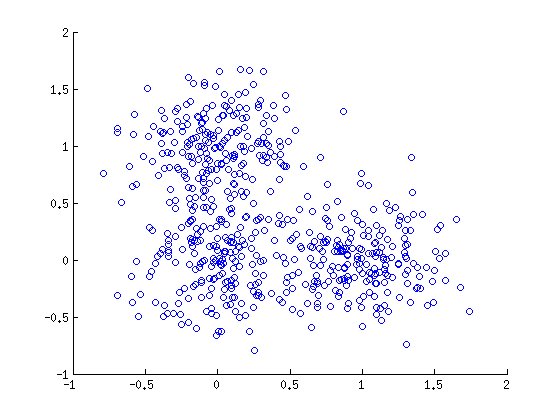
\includegraphics[width=0.35\linewidth]{3gauss} }}
\subfloat[]{{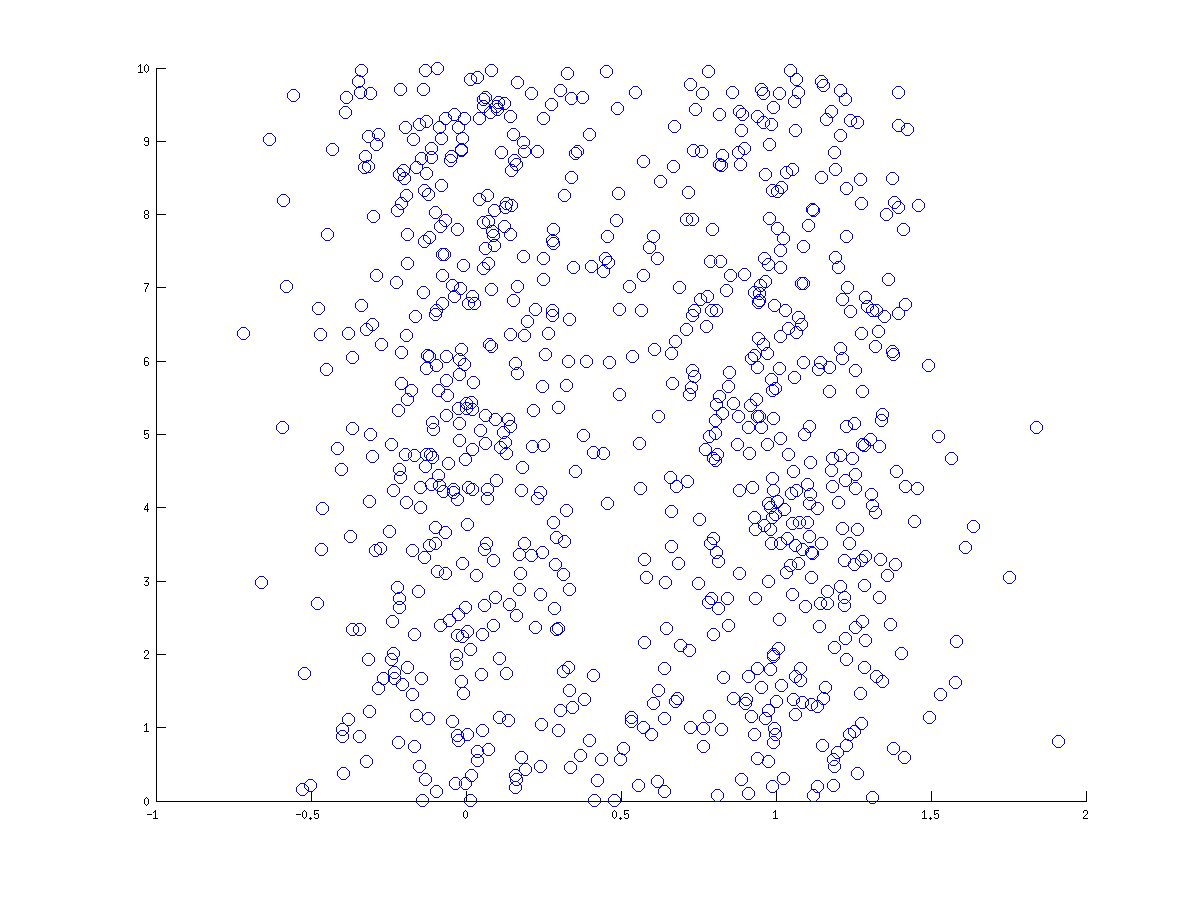
\includegraphics[width=0.35\linewidth]{two_bars} }}
\subfloat[]{{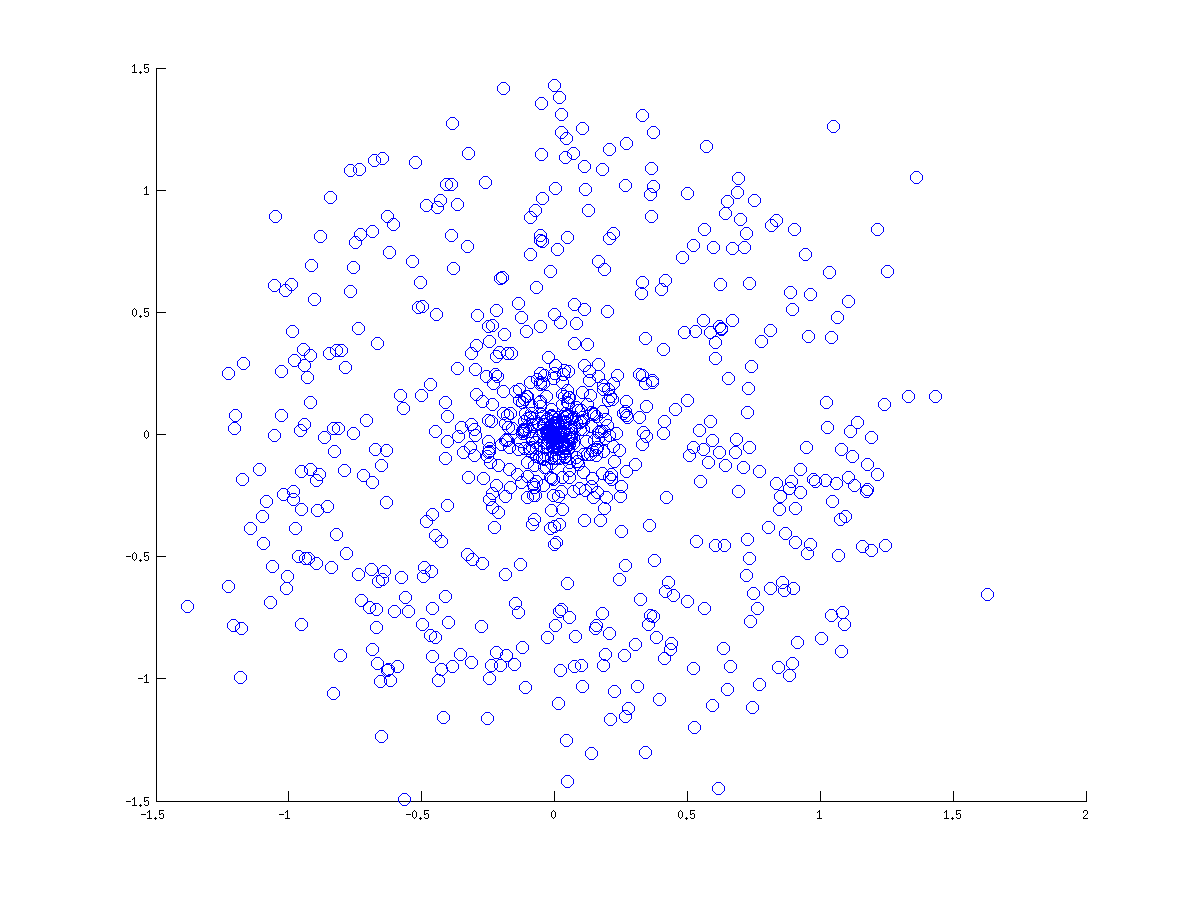
\includegraphics[width=0.35\linewidth]{con_circles} }}
\caption{Realizations of the synthetic datasets (a) \emph{Gaussians}, (b)
\emph{Bars}, and (c) \emph{Circles}.}
\label{fig:synth_dat}
\end{figure}

\emph{Gaussians:}
100 samples from each of $3$ Gaussians in $\R^3$, with covariance $0.25I$ and
means $(0, 0, 1)$, $(0, 1, 0)$, and $(1, 0, 0)$. All algorithms should perform
well given rather distinct, spherical clusters.

\emph{Bars:}
400 noisy samples $(x_i, y_i)$ from each of two long, vertical lines, where
each $y_i \sim$ Unif$(0, 10)$, $x_1,\dots,x_{200} \sim \mathcal{N}(0, 0.3)$,
and $x_{201},\dots,x_{400} \sim \mathcal{N}(1, 0.3)$. We expect K-means to
perform poorly here because the variance in $y$ is much greater than in $x$,
while only $x$ depends on the cluster.

\emph{Circles:} 600 noisy samples
$(x_i, y_i) = (r_i\cos \theta_i, r_i \sin \theta_i)$ from two concentric
circles, where $\theta_i \sim$ Unif$(0, 2\pi)$,
$r_1,\dots,r_{400} \sim \mathcal{N}(1, 0.25)$, and
$r_{401},\dots,r_{600} \sim \mathcal{N}(2, 0.25)$. Since the clusters are not
linearly separable, we expect $K$-means to perform poorly. In order to show
that, unlike clustering via mutual information maximization, CHMin does not
force clusters to be of equals size, we drew $2/3$ of our samples from the
cluster of smaller radius.

\subsubsection{Real Datasets}
\emph{Iris:} $50$ samples of flower measurements from each of $3$ species of
irises.

\emph{Wine:} $178$ samples of each of $13$ chemical properties from wines from
$3$ Italian wine cultivars. Due to the large number of features relative to the
sample size (for a nonparametric method), we expect the kernel density
estimation step may cause CHMin may perform poorly.

\emph{Wine5:} A subset of \emph{Wine} using the (arbitrarily chosen) first $5$
features and all $178$ data points. This subset is used to study how the
performance of CHMin scales with the dimension of the data.

\subsection{Results}
\begin{table}
\small
\centering
\begin{tabular}{c|c|c|c|c|c}
Dataset (\# clusters)   & CHMin                         & K-means++     & HC (single)   & HC (complete) & HC (average)  \\
\hline
Gaussians (3)           & $0.991 \pm 0.008$             & {\bf 0.998}   & 0.767         & 0.984         & 0.994         \\
Bars (2)                & $\mathbf{0.723} \pm 0.013$    & 0.520         & 0.502         & 0.524         & 0.524         \\
Circles (2)             & $\mathbf{0.894} \pm 0.019$    & 0.671         & 0.501         & 0.677         & 0.605         \\
Iris (3)                & $\mathbf{0.929} \pm 0.031$    & 0.893         & 0.680         & 0.840         & 0.906         \\
Wine (3)                & $0.675 \pm 0.0283$            & {\bf 0.702}   & 0.427         & 0.674         & 0.612         \\
Wine5 (3)               & $\mathbf{0.704} \pm 0.044$    & 0.494         & 0.387         & 0.500         & 0.500
\end{tabular}
\caption{Mean ($\pm$ standard deviation) of accuracy, for each algorithm on
each \emph{dataset} (\# of clusters). Hierarchical clustering algorithms are
denoted HC (type), where type is the linkage procedure used. Means and standard
deviations were computed from 100 trials, with synthetic datasets resampled in
each trial. Boldface numbers indicate the best performing algorithm for each
dataset.}
\label{tab:results}
\end{table}

Of the five algorithms tested, CHMin performed best on 4 of 6 datasets. On
the remaining two datasets (\emph{Gaussians} and \emph{Wine}), K-means++
performed best. Since \emph{Gaussians} is precisely the scenario for which
K-means is designed, this is unsurprising. We suspect the poor behavior of
CHMin on \emph{Wine} is due to the poor dependence of kernel density estimation
on dimension (the curse of dimensionality). This is supported by the fact that
the performance of CHMin improved when the number of features was reduced to 5,
while performance of other algorithms fell sharply. For both \emph{Gaussians}
and \emph{Wine}, CHMin still performed competitively (within $3\%$ of K-means).

\section{Conclusions}
In this work, we motivated estimated conditional entropy minimization as a
clustering objective using MDL, proposed a principle for estimaing the number
of clusters based on MDL, proposed CHMin for minimizing the conditional entropy
objective via kernel density estimation and gradient descent, related
CHMin to the $K$-means algorithm, and tested CHMin on real and synthetic data.

Avenues for empirical future work include testing CHMin on larger datasets,
combining CHMin with dimension reduction techniques for high-dimensional
datasets, testing how well our MDL criterion (Theorem 3) can estimate the
number of clusters, and comparing CHMin to more modern nonparametric clustering
approaches such as mutual information maximization, the mean shift algorithm,
the $k$-nearest neighbor approach of \cite{steeg2013demystifying}, and spectral
clustering. Theoretical extensions might include weakening the assumptions of
Theorem 2 to cover the nonparametric case and trying to adapt error bounds
for entropy estimation (see, e.g., \cite{singh14densityfunc}) to study the
performance of CHMin.

\bibliographystyle{unsrt}
\bibliography{project}

\end{document}
